\documentclass{article}
\usepackage[utf8]{inputenc}
\usepackage{hyperref}
\usepackage{amsmath}
\usepackage{amsfonts}
\usepackage{graphicx}
\usepackage{enumitem}
\usepackage{wrapfig}
\graphicspath{ {./images} }


\title{IPhO Class}
\author{
    Tan Chien Hao\\
    \texttt{www.tchlabs.net}\\
    \texttt{Telegram @tch1001}
    % new collaborators add your name and contact here!
}

\date{\today}
\begin{document}
\newif\ifpaper

% TOGGLE ANSWER HERE
\paperfalse 

\maketitle
\tableofcontents
\clearpage 
\section{Mechanics}
\subsection{Over a Wall}
A pump on the ground, $3.0 \mathrm{~m}$ away from a vertical wall of height $4.0 \mathrm{~m}$, ejects water at a velocity $v_0$ at an angle $\theta$ to the horizontal so that it just clears the wall.
\begin{figure}[h]
    \centering
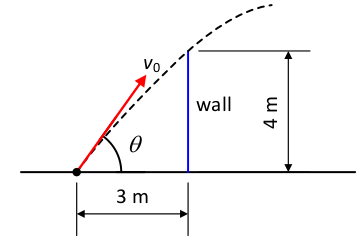
\includegraphics[width=0.5\linewidth]{images/overthewall.png}
\end{figure}
\noindent Determine the minimum value of $v_0$ and the corresponding angle $\theta$. \\[10pt]
Ans: $71.6^\circ$ $9.4 \mathrm{~m} \mathrm{~s}^{-1}$ 
\subsection{Over a Wall Solution}
$$
\begin{aligned}
& y(t)=v_0 \sin \theta t-\frac{1}{2} g t^2 \\
& x(t)=v_0 \cos \theta t . \\
& t(x)=\frac{x}{v_0 \cos \theta} \\
& y(x)=v_0 \sin \theta \frac{x}{v_0 \cos \theta}-\frac{1}{2} g\left(\frac{x}{v_0 \cos \theta}\right)^2 \\
& y(x)=x \tan \theta-\frac{g}{2 v_0} \sec ^2 \theta x^2
\end{aligned}
$$
$y(x)$ passes through $(3,4)$
\begin{align}
4= & 3 \tan \theta-4.5 \frac{g}{v_0^2} \sec ^2 \theta \\
v_0^2(\theta) & =\frac{4.5 g \sec ^2 \theta}{3 \tan \theta-4} \\
& =\frac{4.5 g}{(3 \tan \theta-4) \cos ^2 \theta .} \\
& =\frac{4.5 g}{3 \sin \theta \cos \theta-4 \cos ^2 \theta} .
\end{align}
\begin{align}
& \text { Minimize } v_0^2 \Longleftrightarrow \text { Maximize } \frac{3 \sin \theta \cos \theta-4 \cos ^2 \theta} =: f(\theta) \\
& 0=\frac{d f}{d \theta}=3 \cos 2 \theta-8 \cos \theta(-\sin \theta) \\
& =3 \cos 2 \theta+4 \sin 2 \theta \text {. } \\
& \tan 2 \theta=-\frac{3}{4} \text {. } \\
& \theta=71.565^{\circ} \quad(3 \text { dp}) \\
& v_0^2=88.29 \\
& v_0=9.3963 \quad(5 \text { sf }) \text {. } 
\end{align}
\clearpage 
\subsection{2 Bouncing Balls}
Ball 1 and 2 are simultaneously projected horizontally with velocity $v_1$ and $v_2\left(<v_1\right)$, respectively, from a cliff at a height $H$ from the ground as shown in the figure.\\[10pt]
Ball 1 barely cleared a vertical post at a horizontal distance $x_p$ and landed at a point $\mathrm{R}$ on the ground. Ball 2 rebounded off the ground, barely cleared the vertical post and landed at the same point $R$. Paths of ball 1 and 2 are shown in the figure below.
\begin{figure}[h]
    \centering
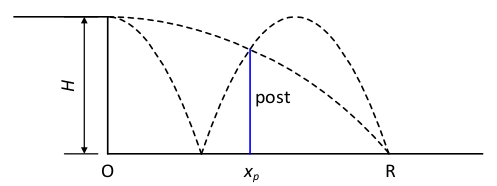
\includegraphics[width=0.8\linewidth]{images/2bouncingballs.png}
\end{figure}
Determine\\[5pt] 
(a) the ratio $v_1 / v_2$, \\[5pt]
(b) the position of the vertical post, and \\[5pt]
(c) the height of the vertical post. 
\clearpage 
\subsection{2 Bouncing Balls Solution}
Ans: (a) 3 (b) $R/2$ (c) $3H/4$
\clearpage 
\subsection{Bouncing Down Stairs}
A marble bounces downstairs in a regular manner, hitting each step at the same place and bouncing the same height above each step.\\[5pt]
The stair height equals its depth (tread=rise) and the coefficient of restitution $e$ is given.\\[5pt]
\begin{figure}[h]
    \centering
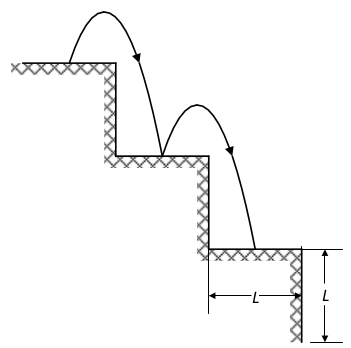
\includegraphics[width=0.8\linewidth]{images/bouncingdownstairs.png}
\end{figure}\\
Determine the necessary horizontal velocity and bounce height.
(The coefficient of restitution is defined as $e=v_f / v_i$ where $v_f$ and $v_i$ are the vertical speeds just after and before the bounce respectively). \\[10pt]
\clearpage
\subsection{Bouncing Down Stairs Solution}
Ans: $v_x=\sqrt{\frac{g L}{2} \cdot \frac{1-e}{1+e}}, H=\frac{e^2 L}{1-e^2}$
\clearpage 
\subsection{Travelling Down Triangle}
The figure shows a right-angle triangle $A B C$ in the vertical plane where $\angle A C B=\theta$. A point mass initially at rest at $A$, reaches $C$ under the influence of gravity via two paths: along $A B$ then $B C$ or along $A C$.\\[10pt]
\begin{figure}[h]
    \centering
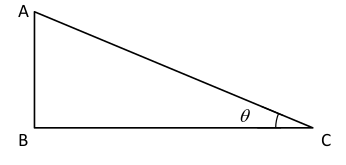
\includegraphics[width=0.8\linewidth]{images/travellingdowntriangle.png}
\end{figure}\\
At any instant, the point mass can instantly change its direction of motion while maintaining the same speed along a horizontal path.\\[10pt]
(a) Determine the angle $\theta$ such that the time taken from $\mathrm{A}$ to $\mathrm{C}$ is the same for both paths.\\[5pt]
(b) For the same angle $\theta$, the point mass can move from $\mathrm{A}$ to $\mathrm{C}$ via a combination of vertical and horizontal motion within ABC. Clearly, there are infinite number of ways this can be achieved. Determine\\[5pt]
(i) the time taken for the path with the longest travelling time,\\[5pt]
(ii) the time taken for the path with the shortest travelling time, and\\[5pt]
(iii) the ratio of these two times.

\clearpage 
\subsection{Travelling Down Triangle Solution}
Ans: $36.8^{\circ}, 2.556 \sqrt{L / g}, 1.826 \sqrt{L / g}, 1.4$
\clearpage
\subsection{Stopping Plane}
A plane landed on a runway with a horizontal velocity of $25 \mathrm{~m} \mathrm{~s}^{-1}$. During taxiing, the plane experienced both drag and lift force of $c_x v^2$ and $c_y v^2$, respectively, where $v$ is the velocity of the plane.\\[10pt]
Suppose $c_x / c_y=0.20$ and the coefficient of friction between the tyres and the runway is $\mu=0.10$, determine the distance the plane travelled on the runway before coming to a stop.
\clearpage
\subsection{Stopping Plane Solution}
Ans: 221 m
\clearpage
\subsection{Engine with Resistance}
An engine of mass $M$ works with a constant tractive force $F$ against a resistance proportional to the square of its speed. The maximum speed it can reach is $U$. Calculate
(a) the time it takes, and
(b) the distance covered, whilst it accelerates from rest to a speed of $\frac{1}{2} U$.
\clearpage 
\subsection{Engine with Resistance Solution}
$$
\left[\frac{m U}{2 F} \ln 3, \frac{m U^2}{2 F} \ln \frac{4}{3}\right]
$$
\clearpage
\subsection{5 Identical Rods}
The figure shows 5 identical uniform rods connected by smooth chains (not shown).
\begin{figure}[h]
    \centering
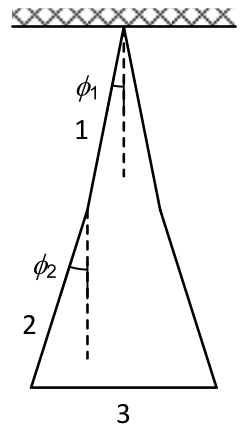
\includegraphics[width=0.4\linewidth]{images/5identicalrods.png}
\end{figure}\\
Determine the angle $\phi_1$ and $\phi_2$.
\clearpage
\subsection{5 Identical Rods Solution}
Ans: $\phi_1=9.869^{\circ}, \phi_2=19.18^{\circ}$
\clearpage
\subsection{Mass on Wedge}
A right-angle smooth wedge of mass $M$ rest on a smooth horizontal plane. The angle of inclination of the wedge is $\theta$. A block of mass $m$, initially at rest on the wedge, is released.
\begin{figure}[h]
    \centering
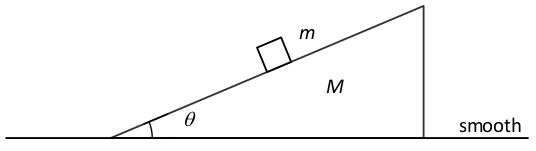
\includegraphics[width=0.8\linewidth]{images/massonwedge.png}
\end{figure}\\
Determine the acceleration of the wedge and the block.
\clearpage
\subsection{Mass on Wedge Solution}
Ans: $\frac{m \sin \theta \cos \theta}{M+m \sin ^2 \theta} \cdot g$
\clearpage
\subsection{Child on Swing }
A child of mass $m$ sits in a swing of negligible mass suspended by a rope of length $L$.
Assume that the dimensions of the child are negligible.
His father pulls him back until the rope makes an angle of one radian with the vertical, then pushes with a force $F=m g$ along the arc of a circle until the rope is vertical and releases the swing.
\begin{figure}[h]
    \centering
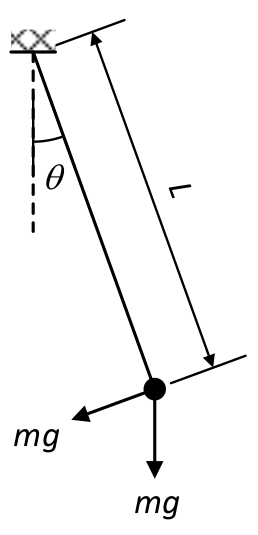
\includegraphics[width=0.3\linewidth]{images/childonswing.png}
\end{figure}\\
For what length of time did the father push the swing?
You may assume that it is sufficiently accurate for this problem to write $\sin \theta \approx \theta$ for $\theta<1$.
\clearpage
\subsection{Child on Swing Solution}
Ans: $t=\frac{\pi}{3} \sqrt{\frac{L}{g}}$
\clearpage
\subsection{Sliding in Bowl }
A point mass undergoes a horizontal circular motion within a hollow sphere of radius $R$. The angle subtended by the point mass about the vertical axis through the centre of the sphere is $\theta$.
\begin{figure}[h]
    \centering
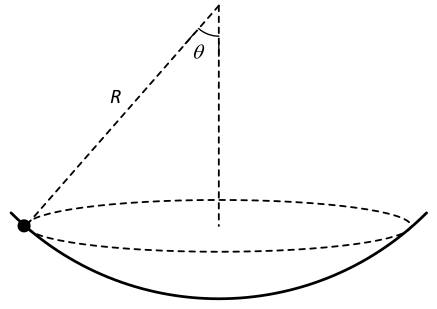
\includegraphics[width=0.6\linewidth]{images/slidinginbowl.png}
\end{figure}\\
Given that the coefficient of friction between the point mass and the wall of the sphere is $\mu$, determine the speed of the ball such that it remains in a fixed position relative to the sphere.

\clearpage
\subsection{Sliding in Bowl Solution}
Ans: $\sqrt{\frac{g(\sin \theta-\mu \cos \theta) R \sin \theta}{\cos \theta+\mu \sin \theta}} \leq v \leq \sqrt{\frac{g(\sin \theta+\mu \cos \theta) R \sin \theta}{\cos \theta-\mu \sin \theta}}$
\clearpage
\subsection{Rolling Collision }
A solid sphere with velocity $u$, rolling on a rough horizontal surface, collides elastically with an identical sphere at rest.
\begin{figure}[h]
    \centering
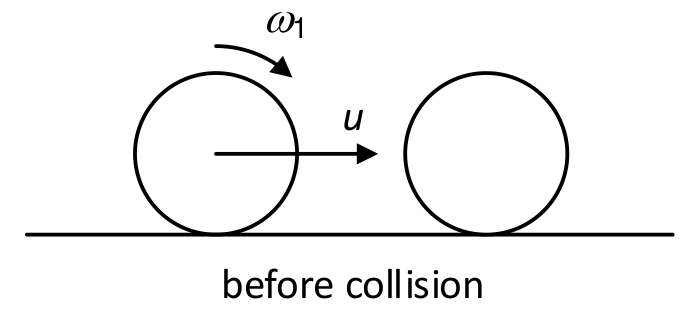
\includegraphics[width=0.6\linewidth]{images/rollingcollision.png}
\end{figure}\\
Assume that the time of collision is very short such that the friction can be ignored during collision. Determine\\
\noindent (a) the velocities of the spheres when both achieved pure rolling motion,\\
\noindent (b) the fractional loss in kinetic energy.

\clearpage
\subsection{Rolling Collision Solution}
Ans: $\frac{2}{7} u, \frac{5}{7} u, 41 \%$
\clearpage
\subsection{Pulling a Reel }
A reel is made up of a hub of radius $R$ and two end caps of radius $r$. The mass of the complete reel is $m$ and its moment of inertia about its longitudinal axis is $I$. The reel rests on a perfectly rough table (so that only rolling motion is possible) and a tension $T$ is applied to the free end of the cotton wrapped around the hub.\\
\begin{figure}[h]
    \centering
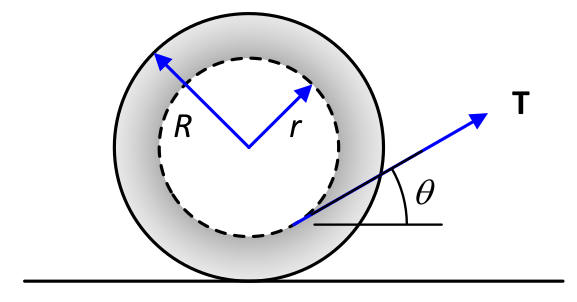
\includegraphics[width=0.6\linewidth]{images/pullingareel.png}
\end{figure}\\
\noindent (a) Describe the linear and angular motion of the reel for small $\theta$ and large $\theta$.\\
\noindent (b) Determine the minimum coefficient of friction so that pure rolling is maintained\\
\noindent (c) If the coefficient of friction is lower than in (b), determine the range of angle where the reel has an acceleration to the right and clockwise angular acceleration.
\clearpage
\subsection{Pulling a Reel Solution}
Ans: $\frac{m R r+l \cos \theta}{\left(I+m R^2\right)(m g-T \sin \theta)} \cdot T,\quad \theta<\sin ^{-1}\left(\frac{m g}{T}-\frac{r}{\mu R}\right)$
\clearpage
\subsection{Ball Hits Ledge }
A uniform cylinder of radius $R$ rolls on a horizontal floor with speed $v_0$ and collides inelastically with a step of height $h$ as shown.
\begin{figure}[h]
    \centering
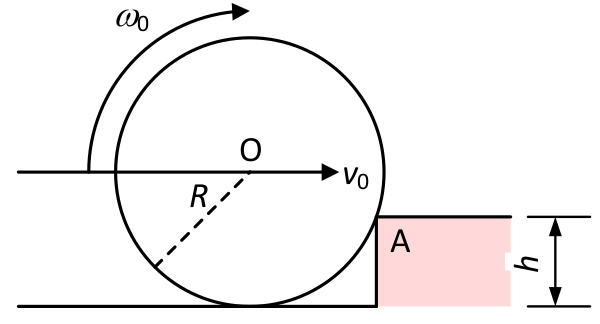
\includegraphics[width=0.6\linewidth]{images/ballhitsledge.png}
\end{figure}\\
Assume that the coefficient of friction is sufficiently large. Determine\\
\noindent (a) the speed of the cylinder such that it rolls up the step without losing contact with the corner A.\\
\noindent (b) the maximum height of the step.

\clearpage
\subsection{Ball Hits Ledge Solution}
Ans: $\frac{3}{7} R$ 
\clearpage
\subsection{Colliding Rods }
On a smooth horizontal table lies two uniform road $\mathrm{A}$ and $\mathrm{B}$ of the same length $L$ and masses $M_A$ and $M_B$, respectively. Rod $\mathrm{A}$ is at rest along the $\mathrm{x}$-axis from $(-L+\varepsilon, \varepsilon)$ where $\varepsilon$ is small. Rod $\mathrm{B}$, lying parallel to the $\mathrm{x}$ axis and occupying the region from $(0, L)$ moves with velocity $v_0$ as shown in the diagram.
\begin{figure}[h]
    \centering
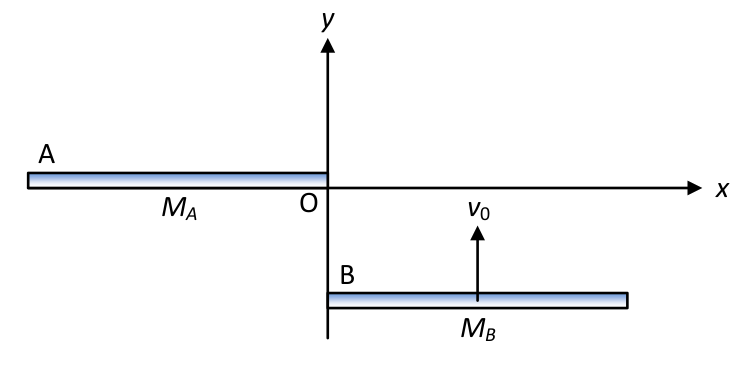
\includegraphics[width=0.6\linewidth]{images/collidingrods.png}
\end{figure}\\
The moment rod $B$ arrives at the $x$-axis, its left edge collides elastically with the right edge of rod $A$. For rod $\mathrm{A}$ and $\mathrm{B}$, determine the respective velocities of each $\mathrm{CM}, v_{\mathrm{A}}$ and $v_B$, and angular velocities, $\omega_A$ and $\omega_B$.

\clearpage
\subsection{Colliding Rods Solution}
\begin{align}
v_A &=\frac{M_B}{2\left(M_A+M_B\right)} v_0 \\
v_B &=\frac{M_A+2 M_B}{2\left(M_A+M_B\right)} v_0 ; \\
\omega_A &=\frac{3 M_B}{\left(M_A+M_B\right) L} v_0 ; \\
\omega_B &=\frac{3 M_A}{\left(M_A+M_B\right) L} v_0
\end{align}
\clearpage
\subsection{Moving Target }
A horizontal circular platform of radius $R$ is rotating with angular velocity $\omega$ about a vertical axis through its centre $\mathrm{O}$. A shooter is positioned at $\mathrm{A}$ at the edge of the platform. He fires a bullet towards a target at $\mathrm{B}$ on the edge of the platform such that $A O B$ is a straight line. The bullet leaves the pistol with a horizontal velocity $u$ relative to the platform.
\begin{figure}[h]
    \centering
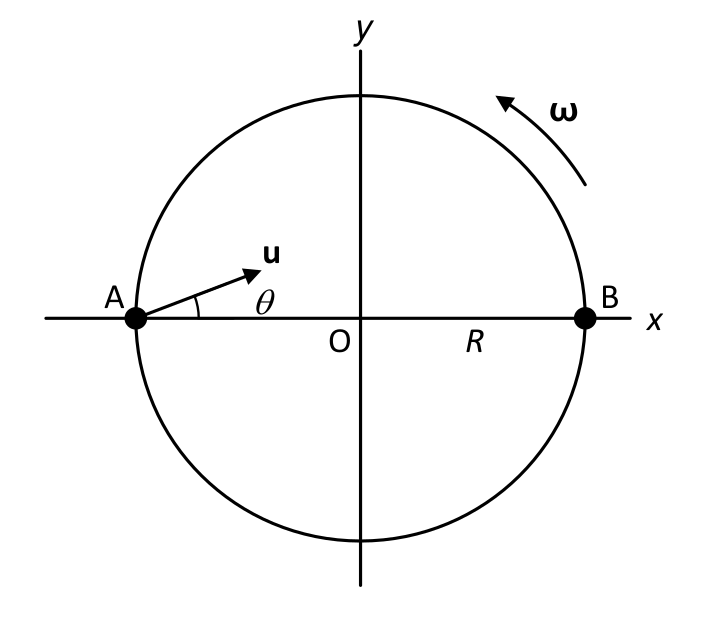
\includegraphics[width=0.5\linewidth]{images/movingtarget.png}
\end{figure}\\
Neglect air resistance.\\
\noindent (a) Determine the direction which the shooter has to aim,\\
\noindent (b) In the frame of the shooter, derive an equation for the path of the bullet.

\clearpage
\subsection{Moving Target Solution}
\begin{align}
\sin ^{-1} \frac{2 \omega R}{u} \\
x^2+\left(y+\sqrt{\left(\frac{u}{2 \omega}\right)^2-R^2}\right)^2=\frac{u^2}{4 \omega^2}
\end{align}
\clearpage
\subsection{Sliding Up Slope }
A uniform solid sphere is projected with speed $V$ and without rotation up a line of greatest slope of a rough plane of inclination $\alpha$. The coefficient of kinetic friction is $\frac{1}{7} \tan \alpha$.\\[20pt]
Show that the friction acts down the plane for a time $t=2 V / 3 g \sin \alpha$ and that afterwards it acts up the plane but is insufficient to prevent slipping.
\clearpage
\subsection{Sliding Up Slope Solution}
\clearpage
\subsection{Midair Exchange }
A straight uniform rigid hair lies on a smooth table; at each end of the hair sits a flea. Show that if the mass $M$ of the hair is not too great relative to that $m$ of each of the fleas, they can, by simultaneous jumps with the same speed and angle of take-off, exchange ends without colliding in mid-air.

\clearpage
\subsection{Midair Exchange Solution}
Ans: $m>M / 6$
\clearpage
\subsection{Ball Hitting Other End }
A uniform rod $A B$ of mass $M$ rests on a smooth horizontal table. A light spring attached to end $B$ of the rod ejects a small ball of mass $m$ with a speed $v$ and at an angle $\theta$ to the rod as shown in the figure (top view).
\begin{figure}[h]
    \centering
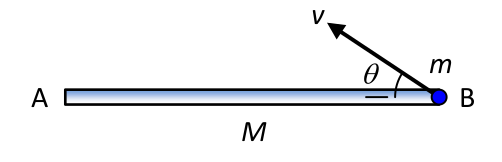
\includegraphics[width=0.5\linewidth]{images/ballhittingotherend.png}
\end{figure}\\
Determine the values of the ratio $\gamma=M / m$ and $\theta$ such that the ball will meet end $A$ of the rod (rotation of the rod is less than $\pi$.)

\clearpage
\subsection{Ball Hitting Other End Solution}
Ans: $0<\gamma<2,65.3^{\circ}>\theta>0$
\clearpage
\subsection{Sandwiched Ball }
A rough plank is hinged to a rough wall at $A$.
When the angle between the plank and the wall is $15^{\circ}$, a wooden cylinder (with an arrow marking its angular displacement) is placed between the plank and the wall as shown.
\begin{figure}[h]
    \centering
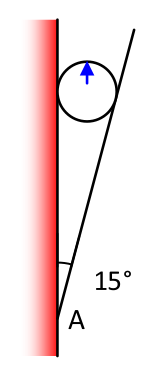
\includegraphics[width=0.5\linewidth]{images/sandwichedball.png}
\end{figure}\\
An external force $\mathbf{F}$ applied normally on the plank keeps the system in equilibrium.
Given that the coefficient of static friction between the cylinder and the wall is 1 and that between the cylinder and the plank is $\sqrt{1 / 3}$, determine the angular displacement of the cylinder when the angle between the plank and the wall is gradually increase to $60^{\circ}$.
\clearpage
\subsection{Sandwiched Ball Solution}
Ans: $135^{\circ}$ clockwise
\clearpage
\subsection{3 Balls }
The figure shows an arrangement of three identical smooth cylinders, of mass $m$ and radius $r$, within a large smooth hollow cylinder of radius $R$.
\begin{figure}[h]
    \centering
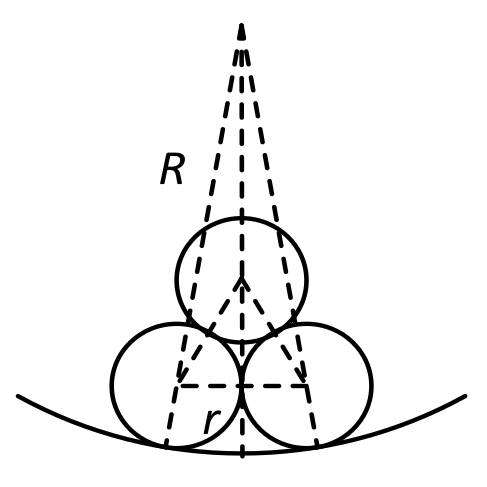
\includegraphics[width=0.5\linewidth]{images/3balls.png}
\end{figure}\\
Show that the maximum radius of the hollow cylinder is $(1+2 \sqrt{7}) r$.
\clearpage
\subsection{3 Balls Solution}
\clearpage
\subsection{}
\clearpage
\subsection{Solution}
\clearpage
\subsection{}
\clearpage
\subsection{Solution}
\clearpage
\subsection{}
\clearpage
\subsection{Solution}
\clearpage
\subsection{}
\clearpage
\subsection{Solution}
\clearpage
\subsection{}
\clearpage
\subsection{Solution}
\clearpage
\subsection{}
\clearpage
\subsection{Solution}
\clearpage
\subsection{}
\clearpage
\subsection{Solution}
\clearpage
\subsection{}
\clearpage
\subsection{Solution}
\clearpage
\subsection{}
\clearpage
\subsection{Solution}
\clearpage
\subsection{}
\clearpage
\subsection{Solution}
\clearpage
\subsection{}
\clearpage
\subsection{Solution}
\clearpage
\subsection{}
\clearpage
\subsection{Solution}
\clearpage
\subsection{}
\clearpage
\subsection{Solution}
\clearpage
\subsection{}
\clearpage
\subsection{Solution}
\clearpage
\subsection{}
\clearpage
\subsection{Solution}
\clearpage
\subsection{}
\clearpage
\subsection{Solution}
\clearpage
\subsection{}
\clearpage
\subsection{Solution}

\end{document}